\documentclass[12pt,letterpaper]{article}
\usepackage{graphicx,textcomp}
\usepackage{natbib}
\usepackage{setspace}
\usepackage{fullpage}
\usepackage{color}
\usepackage[reqno]{amsmath}
\usepackage{amsthm}
\usepackage{fancyvrb}
\usepackage{amssymb,enumerate}
\usepackage[all]{xy}
\usepackage{endnotes}
\usepackage{lscape}
\newtheorem{com}{Comment}
\usepackage{float}
\usepackage{hyperref}
\newtheorem{lem} {Lemma}
\newtheorem{prop}{Proposition}
\newtheorem{thm}{Theorem}
\newtheorem{defn}{Definition}
\newtheorem{cor}{Corollary}
\newtheorem{obs}{Observation}
\usepackage[compact]{titlesec}
\usepackage{dcolumn}
\usepackage{tikz}
\usetikzlibrary{arrows}
\usepackage{multirow}
\usepackage{subcaption}
\usepackage{xcolor}
\newcolumntype{.}{D{.}{.}{-1}}
\newcolumntype{d}[1]{D{.}{.}{#1}}
\definecolor{light-gray}{gray}{0.65}
\usepackage{url}
\usepackage{listings}
\usepackage{color}
\usepackage{mathtools} 
\usepackage{amsmath}
\usepackage{amssymb}
\usepackage{color,soul}

\definecolor{codegreen}{rgb}{0,0.6,0}
\definecolor{codegray}{rgb}{0.5,0.5,0.5}
\definecolor{codepurple}{rgb}{0.58,0,0.82}
\definecolor{backcolour}{rgb}{0.95,0.95,0.92}

\lstdefinestyle{mystyle}{
	backgroundcolor=\color{backcolour},   
	commentstyle=\color{codegreen},
	keywordstyle=\color{magenta},
	numberstyle=\tiny\color{codegray},
	stringstyle=\color{codepurple},
	basicstyle=\footnotesize,
	breakatwhitespace=false,         
	breaklines=true,                 
	captionpos=b,                    
	keepspaces=true,                 
	numbers=left,                    
	numbersep=5pt,                  
	showspaces=false,                
	showstringspaces=false,
	showtabs=false,                  
	tabsize=2
}
\lstset{style=mystyle}
\newcommand{\Sref}[1]{Section~\ref{#1}}

\title{Submission for Problem Set 3}
\date{Duc Minh, VU \\
	TCD StudentID: 22996761 / UCD StudentID: 19211157}
\author{Applied Stats/Quant Methods 1}

\begin{document}
	\maketitle
	\section*{Question 1}
	\noindent The incumbent dataset will first be imported and the relevant library will be loaded in R for analysis.
	\lstinputlisting[language=R, firstline=11, lastline=13]{PS3_answers_Duc Minh, Vu.R}
	\begin{enumerate}
		\item Regression modelling with \textit{\texttt{voteshare}} as the outcome variable and the \textit{\texttt{difflog}} as explanatory variable
		\lstinputlisting[language=R, firstline=16, lastline=21]{PS3_answers_Duc Minh, Vu.R}
		\begin{verbatim}
			Call:
			lm(formula = voteshare ~ difflog, data = incumb_data)
			
			Residuals:
			Min       1Q   Median       3Q      Max 
			-0.26832 -0.05345 -0.00377  0.04780  0.32749 
			
			Coefficients:
			Estimate Std. Error t value Pr(>|t|)    
			(Intercept) 0.579031   0.002251  257.19   <2e-16 ***
			difflog     0.041666   0.000968   43.04   <2e-16 ***
			---
			Signif. codes:  0 ‘***’ 0.001 ‘**’ 0.01 ‘*’ 0.05 ‘.’ 0.1 ‘ ’ 1
			
			Residual standard error: 0.07867 on 3191 degrees of freedom
			Multiple R-squared:  0.3673,	Adjusted R-squared:  0.3671 
			F-statistic:  1853 on 1 and 3191 DF,  p-value: < 2.2e-16
		\end{verbatim}
		\begin{table}[H]
			\begin{center}
				\begin{tabular}{l c}
					\hline
					& Model 1 \\
					\hline
					(Intercept) & $0.5790^{***}$ \\
					& $(0.0023)$     \\
					difflog     & $0.0417^{***}$ \\
					& $(0.0010)$     \\
					\hline
					R$^2$       & $0.3673$       \\
					Adj. R$^2$  & $0.3671$       \\
					Num. obs.   & $3193$         \\
					\hline
					\multicolumn{2}{l}{\scriptsize{$^{***}p<0.001$; $^{**}p<0.01$; $^{*}p<0.05$}}
				\end{tabular}
				\caption{Vote share (voteshare) and log differences in campaign spending (difflog)}
				\label{table:coefficients}
			\end{center}
		\end{table}
	There is statistical evidence that there is a positive relationship between incumbent's voteshare and the difference in campaign spending between incumbent and challenger. For a one unit increase in the logged difference in spending, the incumbent's voteshare is predicted to increase, on average, by 0.04.
	
		\item Create a scatterplot for the two variables
		\lstinputlisting[language=R, firstline=27, lastline=31]{PS3_answers_Duc Minh, Vu.R}
		\begin{figure}[H]\centering
			\caption{\footnotesize Scatterplot between voteshare and difflog}
			\label{fig:plot_1}
			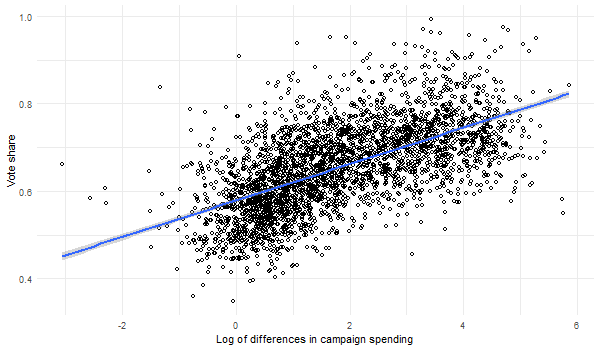
\includegraphics[width=.85\textwidth]{1.2. Scatter_plot_voteshare_difflog.png}
		\end{figure}
	
		\item Save the residuals
		\lstinputlisting[language=R, firstline=35, lastline=35]{PS3_answers_Duc Minh, Vu.R}
		
		\item Prediction equation
		$$\hat{y} = \hat{\beta\textsubscript{0}} + \hat{\beta\textsubscript{1}} \times \textit{x} $$
		$$ \textit{\texttt{voteshare}} = 0.579 + 0.042 \times \textit{\texttt{difflog}}$$
	\end{enumerate}

	\section*{Question 2}
	\begin{enumerate}
		\item Regression modelling with \textit{\texttt{presvote}} as the outcome variable and the \textit{\texttt{difflog}} as explanatory variable
		\lstinputlisting[language=R, firstline=41, lastline=46]{PS3_answers_Duc Minh, Vu.R}
		\begin{verbatim}
			lm(formula = presvote ~ difflog, data = incumb_data)
			
			Residuals:
			Min       1Q   Median       3Q      Max 
			-0.32196 -0.07407 -0.00102  0.07151  0.42743 
			
			Coefficients:
			Estimate Std. Error t value Pr(>|t|)    
			(Intercept) 0.507583   0.003161  160.60   <2e-16 ***
			difflog     0.023837   0.001359   17.54   <2e-16 ***
			---
			Signif. codes:  0 ‘***’ 0.001 ‘**’ 0.01 ‘*’ 0.05 ‘.’ 0.1 ‘ ’ 1
			
			Residual standard error: 0.1104 on 3191 degrees of freedom
			Multiple R-squared:  0.08795,	Adjusted R-squared:  0.08767 
			F-statistic: 307.7 on 1 and 3191 DF,  p-value: < 2.2e-16
		\end{verbatim}
		\begin{table}[H]
			\begin{center}
				\begin{tabular}{l c}
					\hline
					& Model 2 \\
					\hline
					(Intercept) & $0.5076^{***}$ \\
					& $(0.0032)$     \\
					difflog     & $0.0238^{***}$ \\
					& $(0.0014)$     \\
					\hline
					R$^2$       & $0.0880$       \\
					Adj. R$^2$  & $0.0877$       \\
					Num. obs.   & $3193$         \\
					\hline
					\multicolumn{2}{l}{\scriptsize{$^{***}p<0.001$; $^{**}p<0.01$; $^{*}p<0.05$}}
				\end{tabular}
				\caption{Vote share of presidental candidate (presvote) and log differences in campaign spending (difflog)}
				\label{table:coefficients}
			\end{center}
		\end{table}
	There is statistical evidence that there is a postive relationship between vote share of the presidential candidate and the difference in spending between incumbent and challengers. For a one unit increase in the logged difference in spending, the incumbent's voteshare of the presidential candidate is predicted to increase, on average, by 0.0238.
	
		\item Create a scatterplot for the two variables
			\lstinputlisting[language=R, firstline=52, lastline=56]{PS3_answers_Duc Minh, Vu.R}
			\begin{figure}[H]\centering
				\caption{\footnotesize Scatterplot between presvote and difflog}
				\label{fig:plot_1}
				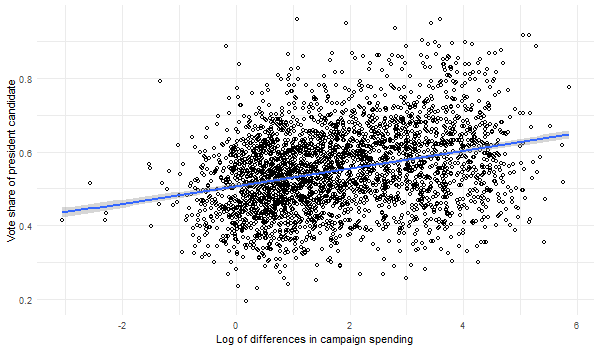
\includegraphics[width=.85\textwidth]{2.2. Scatter_plot_presvote_difflog.png}
			\end{figure}
		
		\item Save the residuals
			\lstinputlisting[language=R, firstline=60, lastline=60]{PS3_answers_Duc Minh, Vu.R}
			
		\item Prediction equation
		$$\hat{y} = \hat{\beta\textsubscript{0}} + \hat{\beta\textsubscript{1}} \times \textit{x} $$
		$$ \textit{\texttt{presvote}} = 0.5076 + 0.0238 \times \textit{\texttt{difflog}}$$
	\end{enumerate}

	\section*{Question 3}
	\begin{enumerate}
		\item Regression modelling with \textit{\texttt{voteshare}} as the outcome variable and the \textit{\texttt{presvote}} as explanatory variable
		\lstinputlisting[language=R, firstline=66, lastline=71]{PS3_answers_Duc Minh, Vu.R}
		\begin{verbatim}
			lm(formula = voteshare ~ presvote, data = incumb_data)
			
			Residuals:
			Min       1Q   Median       3Q      Max 
			-0.27330 -0.05888  0.00394  0.06148  0.41365 
			
			Coefficients:
			Estimate Std. Error t value Pr(>|t|)    
			(Intercept) 0.441330   0.007599   58.08   <2e-16 ***
			presvote    0.388018   0.013493   28.76   <2e-16 ***
			---
			Signif. codes:  0 ‘***’ 0.001 ‘**’ 0.01 ‘*’ 0.05 ‘.’ 0.1 ‘ ’ 1
			
			Residual standard error: 0.08815 on 3191 degrees of freedom
			Multiple R-squared:  0.2058,	Adjusted R-squared:  0.2056 
			F-statistic:   827 on 1 and 3191 DF,  p-value: < 2.2e-16
		\end{verbatim}
		\begin{table}[H]
			\begin{center}
				\begin{tabular}{l c}
					\hline
					& Model 3 \\
					\hline
					(Intercept) & $0.4413^{***}$ \\
					& $(0.0076)$     \\
					presvote    & $0.3880^{***}$ \\
					& $(0.0135)$     \\
					\hline
					R$^2$       & $0.2058$       \\
					Adj. R$^2$  & $0.2056$       \\
					Num. obs.   & $3193$         \\
					\hline
					\multicolumn{2}{l}{\scriptsize{$^{***}p<0.001$; $^{**}p<0.01$; $^{*}p<0.05$}}
				\end{tabular}
				\caption{Incumbent's electoral success (voteshare) and Vote share of presidental candidate (presvote)}
				\label{table:coefficients}
			\end{center}
		\end{table}
	There is statistical evidence that there is a positive relationship between vote share of the presidential candidate and vote share. For a one unit increase the vote share of the presidential candidate, the incumbent's voteshare is predicted to increase, on average, by 0.388%.
		
		\item Create a scatterplot for the two variables
			\lstinputlisting[language=R, firstline=77, lastline=81]{PS3_answers_Duc Minh, Vu.R}
			\begin{figure}[H]\centering
				\caption{\footnotesize Scatterplot between voteshare and presvote}
				\label{fig:plot_1}
				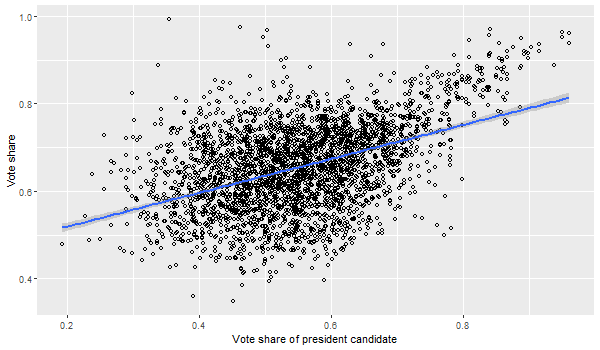
\includegraphics[width=.85\textwidth]{3.2. Scatter_plot_voteshare_presvote.png}
			\end{figure}
		
		\item Prediction equation
		$$\hat{y} = \hat{\beta\textsubscript{0}} + \hat{\beta\textsubscript{1}} \times \textit{x} $$
		$$ \textit{\texttt{voteshare}} = 0.4413 + 0.388 \times \textit{\texttt{presvote}}$$
	\end{enumerate}

	\section*{Question 4}
	\begin{enumerate}
		\item Regression modelling with \texttt{Q1's residuals} as the outcome variable and the \texttt{Q2's residuals} as explanatory variable
			\lstinputlisting[language=R, firstline=88, lastline=93]{PS3_answers_Duc Minh, Vu.R}
			\begin{verbatim}
				lm(formula = vote.lm.resid ~ presvote.lm.resid)
				
				Residuals:
				Min       1Q   Median       3Q      Max 
				-0.25928 -0.04737 -0.00121  0.04618  0.33126 
				
				Coefficients:
				Estimate Std. Error t value Pr(>|t|)    
				(Intercept)      -4.860e-18  1.299e-03    0.00        1    
				presvote.lm.resid  2.569e-01  1.176e-02   21.84   <2e-16 ***
				---
				Signif. codes:  0 ‘***’ 0.001 ‘**’ 0.01 ‘*’ 0.05 ‘.’ 0.1 ‘ ’ 1
				
				Residual standard error: 0.07338 on 3191 degrees of freedom
				Multiple R-squared:   0.13,	Adjusted R-squared:  0.1298 
				F-statistic:   477 on 1 and 3191 DF,  p-value: < 2.2e-16
			\end{verbatim}
			\begin{table}[H]
				\begin{center}
					\begin{tabular}{l c}
						\hline
						& Model 4 \\
						\hline
						(Intercept)      & $-0.0000$      \\
						& $(0.0013)$     \\
						presvote.lm.resid & $0.2569^{***}$ \\
						& $(0.0118)$     \\
						\hline
						R$^2$            & $0.1300$       \\
						Adj. R$^2$       & $0.1298$       \\
						Num. obs.        & $3193$         \\
						\hline
						\multicolumn{2}{l}{\scriptsize{$^{***}p<0.001$; $^{**}p<0.01$; $^{*}p<0.05$}}
					\end{tabular}
					\caption{Question 1 residuals (vote.lm.resid) and Question 2 residuals (presvote.lm.resid)}
					\label{table:coefficients}
				\end{center}
			\end{table}
		There is statistical evidence that there is a positive relationship between residuals from Question 1 and residuals from Question 2. For a one unit increase the residuals from question 1, the residuals from question 2 is predicted to increase, on average, by 0.2569.
		
		\item Create a scatterplot for the two variables
			\lstinputlisting[language=R, firstline=99, lastline=101]{PS3_answers_Duc Minh, Vu.R}
			\begin{figure}[H]\centering
				\caption{\footnotesize Scatterplot between residuals from Question 1 and 2}
				\label{fig:plot_1}
				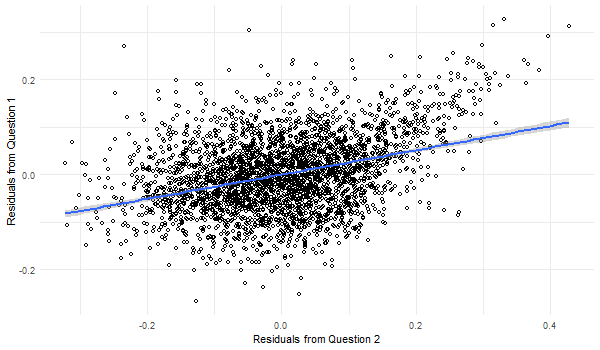
\includegraphics[width=.85\textwidth]{4.2. Scatter_plot_residuals.png}
			\end{figure}
		
		\item Prediction equation
		$$\hat{y} = \hat{\beta\textsubscript{0}} + \hat{\beta\textsubscript{1}} \times \textit{x} $$
		$$\text{Q1's residuals} = \hat{\beta\textsubscript{0}} + \hat{\beta\textsubscript{1}} \times \text{Q2's residuals} $$
		$$ \textit{\texttt{vote.lm.resid}} = 0 + 0.2569 \times \textit{\texttt{presvote.lm.resid}}$$
	\end{enumerate}

	\section*{Question 5}
	\begin{enumerate}
		\item Regression modelling with \textit{\texttt{voteshare}} as the outcome variable and, \textit{\texttt{difflog}} and \textit{\texttt{presvote}} as explanatory variables
			\lstinputlisting[language=R, firstline=110, lastline=115]{PS3_answers_Duc Minh, Vu.R}
			\begin{verbatim}
				lm(formula = voteshare ~ difflog + presvote, data = incumb_data)
				
				Residuals:
				Min       1Q   Median       3Q      Max 
				-0.25928 -0.04737 -0.00121  0.04618  0.33126 
				
				Coefficients:
				Estimate Std. Error t value Pr(>|t|)    
				(Intercept) 0.4486442  0.0063297   70.88   <2e-16 ***
				difflog     0.0355431  0.0009455   37.59   <2e-16 ***
				presvote    0.2568770  0.0117637   21.84   <2e-16 ***
				---
				Signif. codes:  0 ‘***’ 0.001 ‘**’ 0.01 ‘*’ 0.05 ‘.’ 0.1 ‘ ’ 1
			\end{verbatim}
			\begin{table}[H]
				\begin{center}
					\begin{tabular}{l c}
						\hline
						& Model 5 \\
						\hline
						(Intercept) & $0.4486^{***}$ \\
						& $(0.0063)$     \\
						difflog     & $0.0355^{***}$ \\
						& $(0.0009)$     \\
						presvote    & $0.2569^{***}$ \\
						& $(0.0118)$     \\
						\hline
						R$^2$       & $0.4496$       \\
						Adj. R$^2$  & $0.4493$       \\
						Num. obs.   & $3193$         \\
						\hline
						\multicolumn{2}{l}{\scriptsize{$^{***}p<0.001$; $^{**}p<0.01$; $^{*}p<0.05$}}
					\end{tabular}
					\caption{Vote shares (voteshare) with difference in spending (difflog) and president's popularity (presvote)}
					\label{table:coefficients}
				\end{center}
			\end{table}
		
		\item Prediction equation
		$$\hat{y} = \hat{\beta\textsubscript{0}} + \hat{\beta\textsubscript{1}} \times \textit{x}\textsubscript{1} +\hat{\beta\textsubscript{2}} \times \textit{x}\textsubscript{2} $$
		$$ \textit{\texttt{voteshare}} = 0.4486 + 0.0355 \times \textit{\texttt{difflog}} + 0.2569 \times \textit{\texttt{presvote}} $$
		
		\item Comparison
		\lstinputlisting[language=R, firstline=118, lastline=121]{PS3_answers_Duc Minh, Vu.R}
		\begin{table}[H]
			\begin{center}
				\begin{tabular}{l c c}
					\hline
					& Model 4 & Model 5 \\
					\hline
					(Intercept)      & $-0.0000$      & $0.4486^{***}$ \\
					& $(0.0013)$     & $(0.0063)$     \\
					presvote.lm.resid & $0.2569^{***}$ &                \\
					& $(0.0118)$     &                \\
					difflog          &                & $0.0355^{***}$ \\
					&                & $(0.0009)$     \\
					presvote         &                & $0.2569^{***}$ \\
					&                & $(0.0118)$     \\
					\hline
					R$^2$            & $0.1300$       & $0.4496$       \\
					Adj. R$^2$       & $0.1298$       & $0.4493$       \\
					Num. obs.        & $3193$         & $3193$         \\
					\hline
					\multicolumn{3}{l}{\scriptsize{$^{***}p<0.001$; $^{**}p<0.01$; $^{*}p<0.05$}}
				\end{tabular}
				\caption{Comparison between model from Question 4 and 5}
				\label{table:coefficients}
			\end{center}
		\end{table}
	\hspace*{15pt} From Table 6, we can see that both the coefficients for the residuals \textit{\texttt{presvote.lm.resid}} from Model 4 of Question 4 and \textit{\texttt{presvote}} from Model 5 of Question 5 have the same value of 0.2569.\\
	\hspace*{15pt} First, let's look at the relationships between the three variables \textit{\texttt{presvote}}, \textit{\texttt{voteshare}} and \textit{\texttt{difflog}}. Question 3 shows us that there is a relationship between \textit{\texttt{presvote}} and \textit{\texttt{voteshare}}. But, at the same time, we also know that \textit{\texttt{difflog}} have a relationship with both \textit{\texttt{voteshare}} and \textit{\texttt{presvote}} from Question 1 and 2 respectively. See Figure 5 below which I have constructed manually.\\
	\begin{figure}[H]\centering
		\caption{\footnotesize Graphical depiction of the relationship between \textit{\texttt{voteshare}}, \textit{\texttt{presvote}} and \textit{\texttt{difflog}}}
		\label{fig:plot_1}
		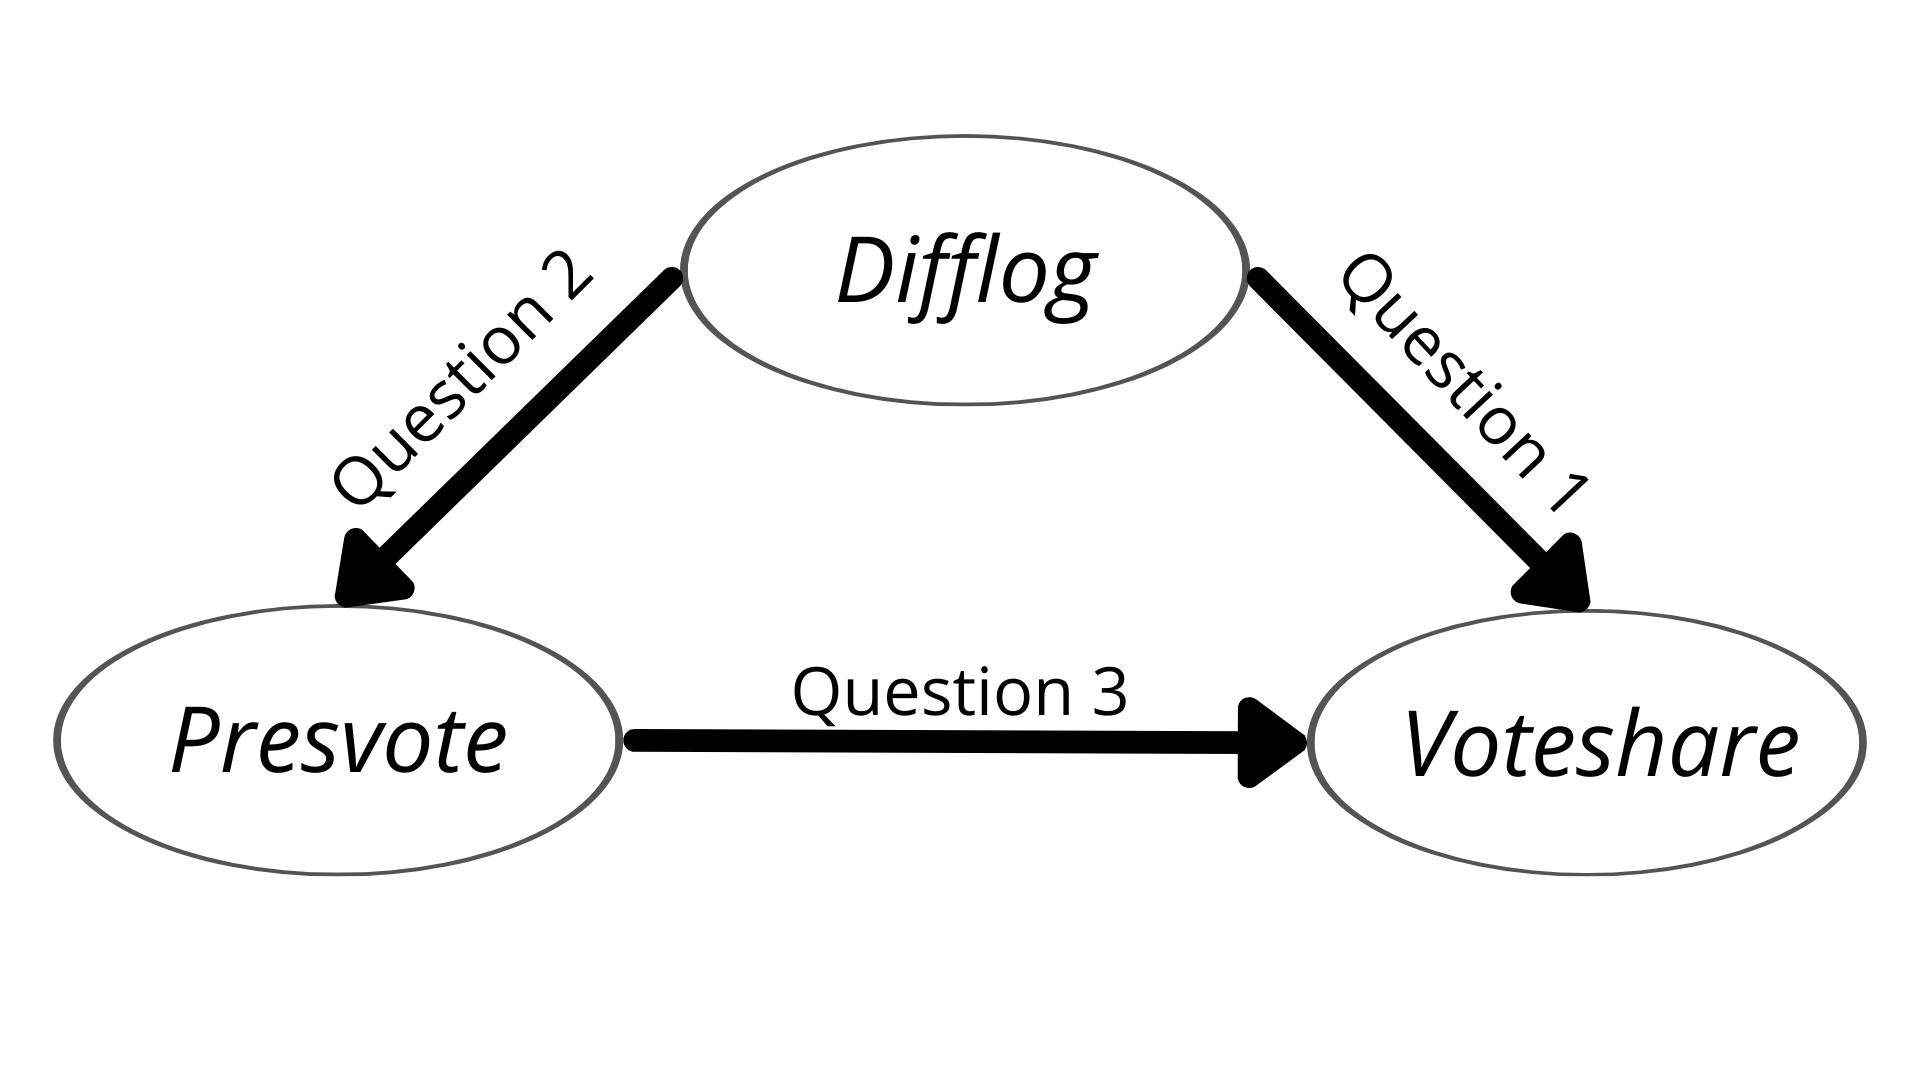
\includegraphics[width=.85\textwidth]{5. Variables relationship.png}
	\end{figure}
	\hspace*{15pt} Hence, when using only \textit{\texttt{presvote}} to predict   \textit{\texttt{voteshare}}, we cannot estimate its "pure" effect on \textit{\texttt{voteshare}}, because there is a shared variance from both \textit{\texttt{presvote}} and \textit{\texttt{difflog}} (due to their relationship) in explaining \textit{\texttt{voteshare}}. Hence, the residuals from Question 1 and 2 provide us with the variance in \textit{\texttt{voteshare}} and \textit{\texttt{presvote}} \textbf{\underline{unexplained}} by \textit{\texttt{difflog}}. In essence, by obtaining the residuals from these bivariate regressions, we have "clean" both \textit{\texttt{voteshare}} and \textit{\texttt{presvote}} of their correlation with \textit{\texttt{difflog}}. Therefore, when we run the bivariate model between these residuals, we are getting the 'pure' (relatively as in not influenced by \textit{\texttt{difflog}}) covaration between \textit{\texttt{voteshare}} and \textit{\texttt{presvote}}.\\
	\hspace*{15pt} This is essentially what multiple regression do as it control for the effects of other variables on the dependent variables. In our case, the influence of \textit{\texttt{difflog}} is controlled for when it has been included into the regression model, so we can get the partial effect of \textit{\texttt{presvote}} only. Hence, this is why we have the same coefficients or to sum up, both the coefficients for the residuals \textit{\texttt{presvote.lm.resid}} from Model 4 of Question 4 and \textit{\texttt{presvote}} from Model 5 of Question 5 show us the partial effect of \textit{\texttt{presvote}}.
	\end{enumerate}
\end{document}